% Overview:
%   Kevlar TeX subfile for the project.
%   Each subfile MUST start with the following line
%		\documentclass[../main.tex]{subfiles}

\documentclass[../main.tex]{subfiles}

\begin{document}

\subsection{Kevlar}
\label{kevlar}

Il primo framework che viene presentato in questa sezione è Kevlar \cite{standage2019kevlar}: si basa su una formulazione \textit{mapping-free} del problema della scoperta delle varianti \textit{de novo}. Intuitivamente, una nuova mutazione cellulare dovrebbe comportare un nuova sequenza nel probando\footnote{\ In genetica umana, il probando è il primo individuo esaminato in cui si riscontra un determinato carattere e dal quale si parte per la costruzione di un albero genealogico che serva a stabilire se il carattere è ereditario e con quale modalità viene trasmesso.} rispetto ai genomi dei genitori. Anche nel caso più semplice, la maggior parte dei \textit{k}-mer della mutazione dovrebbero essere unici, dato un valore sufficientemente grande di \textit{k}. Con un campionamento sufficientemente profondo del genoma del probando, l'aspettativa è che questi nuovi \textit{k}-mer siano frequenti nelle read in modo da essere facilmente distinti dagli errori di sequenziamento. Pertanto, dovrebbe essere possibile rilevare simultaneamente sia SNV che varianti più grandi (indels, SV), utilizzando un singolo modello privo di mappatura.
\\\\
Partendo da questa intuizione, Kevlar esamina la frequenza con cui compaiono i \textit{k}-mer per identificare quali possono essere interessanti\footnote{\ Un \textit{k}-mer è definito interessante se compare frequentemente nel genoma del figlio, ed è del tutto assente dai genomi di entrambi i genitori.}, e usarli come indicatori della potenziale esistenza di mutazioni \textit{de novo} all'interno del genoma figlio. Successivamente, raggruppa i \textit{k}-mer interessanti in insiemi disgiunti e assembla ogni insieme di read in contig, allineandoli ad un genoma di riferimento per effettuare una chiamata alle varianti preliminare. Infine impiega un modello probabilistico per classificare e filtrare le varianti chiamate.

\subsubsection{Algoritmo di Kevlar}

Nella figura \ref{fig:kevlar_pipeline} è riportato il workflow dell'algoritmo di Kevlar e successivamente una breve descrizione dei singoli step.

\begin{figure}[ht!]
	\centering
  	\captionsetup{justification=centering}
  	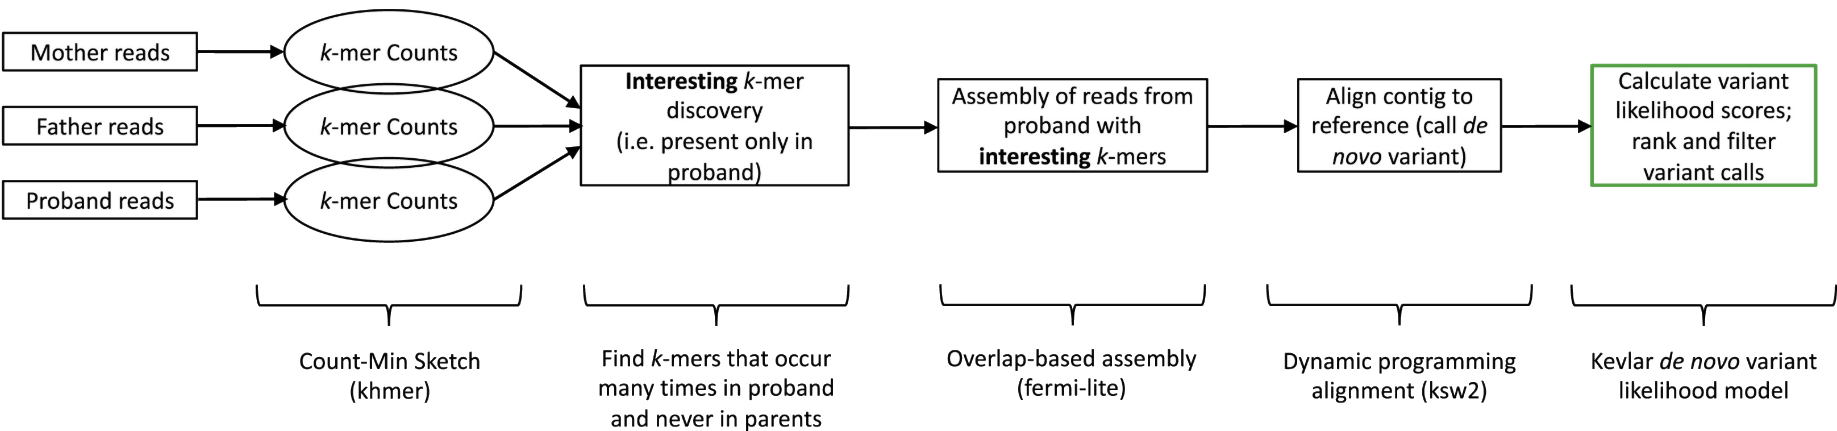
\includegraphics[scale=.27]{images/kevlar_pipeline.png}
  	\caption{}
  	\label{fig:kevlar_pipeline}
\end{figure}

\noindent 
\textbf{Step 1} Prima di poter identificare nuovi \textit{k}-mer, è necessario contare la frequenza di ogni \textit{k}-mer all'interno di ogni genoma. Per fare ciò Kevlar memorizza un conteggio approssimativo dei \textit{k}-mer all'interno di Count-Min sketch, una struttura dati probabilistica simile a un Bloom Filter (vedi Sezione \ref{BloomFilter}) che però opera con una taglia sublineare dell'input, favorendo l'efficienza alla precisione. Viene utilizzata per ogni campione una CM sketch, la cui precisione dipende dalla dimensione e dal numero degli elementi distinti che vengono tracciati. In seguito, con l'utilizzo di una maschera di conteggio, se i \textit{k}-mer sono presenti nei genomi di riferimento e in un genoma di contaminamenti (batteri, virus, ...) sono ignorati.

\paragraph{Step 2} Kevlar scansiona ogni read sequenziata dal probando e richiede le frequenze per campione di ciascun \textit{k}-mer alle Count-Min sketch generate nella fase precedente. Se un \textit{k}-mer è presente con alta frequenza nel genoma figlio ed è assente dai genomi genitori è identificato come "interessante". 

\paragraph{Step 3} Ogni read che contiente \textit{k}-mer interessanti viene filtrata prima di qualunque altra analisi. Questo filtraggio serve principalmente per due scopi. (1) Dato il volume delle read che arriva a questo step, Kevlar è in grado di ricalcolare esattamente le frequenze di ogni \textit{k}-mer interessante nel probando e qualunque \textit{k}-mer il cui conteggio ``corretto'' non soddisfi più la frequenza di soglia viene scartato. (2) Se per qualunque ragione dei \textit{k}-mer presenti nel genoma di riferimento e dei contaminanti non erano stati ignorati nel conteggio iniziale, questo filtraggio fornisce un'altra opportunità per scartarli. 

Dopo l'applicazione di questo filtraggio, qualunque read che non contiene \textit{k}-mer interessanti è scartata. Ci si aspetta ora che read interessanti condividano numerosi \textit{k}-mer interessanti: tramite questi è possibile raggruppare le read interessanti in insiemi disgiunti, ognuno rappresentante una mutazione. Per fare ciò viene definito un grafo di lettura $G$ nel seguente modo: ogni read contenente uno o più \textit{k}-mer interessanti è rappresentata da un nodo in $G$; una coppia di nodi è connessa da un arco se le rispettive read hanno uno o più \textit{k}-mer interessanti in comune. Grazie a questa formulazione, se due read condividono un \textit{k}-mer interessante, allora sono parte della stessa componente connessa di $G$. 

Per ogni componente connessa $p\in G$ viene assemblata la read corrispondente usando un algoritmo basato su overlap, implementato nella libreria Fermi-Lite e viene prodotto il cammino ottimale $C_p$ nel grafo (sottoforma di contig) adatto per effettuare chiamate delle varianti. Vengono successivamente selezionate delle sequenze obiettivo di riferimento per il contig $C_p$ denotate come $T_{C_p}$.

\paragraph{Step 4} Il contig $C_p$ viene allineato a ciascuna sequenza obiettivo $t \in T_{C_p}$ usando la libreria ksw2\footnote{\ ksw2 implementa la formulazione di Green di allineamento ed estensione globale della programmazione dinamica.}. 
Se sono presenti più sequenze obiettivo, viene mantenuto solo l'allineamento con il punteggio più alto. Quando un contig si allinea a più posizioni con lo stesso punteggio ottimale, tutti gli allineamenti ottimali vengono mantenuti per la chiamata della variante.
Prima di chiamare la variante, Kevlar allinea eventuali spazi vuoti all'estremità destra dell'allineamento per ridurre al minimo il numero di operazioni di allineamento. Successivamente, ispeziona il percorso di allineamento (rappresentato come una stringa \texttt{CIGAR}) di ciascun allineamento e verifica la corrispondenza con i pattern previsti. Allineamenti corrispondenti al pattern \verb|ˆ(\d+[DI])?\d+M(\d+[DI])?$| sono classificati come SNV e il blocco ``match" dell'allineamento viene scansionato per discrepanze tra il contig e l'obiettivo di riferimento. Qualsiasi discrepanza è segnalata come variante a singolo nucleotide. Gli allineamenti che corrispondono al pattern \verb|ˆ(\d+[DI])?\d+M\d+[ID]\d+M(\d+[DI])?$| sono invece classificati come indel. Oltre a segnalare il divario interno di questo allineamento come un indel, i blocchi ``match" fiancheggianti sono
scansionati anche per discrepanze tra il contig e il target da segnalare come putativi SNV. Qualsiasi allineamento che non corrisponde ai due pattern sopra descritti è designato come ``\texttt{no-call}'' ovvero non interpretabile, ed elencata nell'output con il contig corrispondente. 

\paragraph{Step 5} 

Per assegnare un punteggio e classificare le mutazioni \textit{de novo}, viene utilizzato un modello probabilistico che considera la frequenza dei \textit{k}-mer interessanti per calcolare la probabilità che siano \textit{de novo}, ereditati o semplicemente dei falsi positivi. Utilizzando queste probabilità, viene calcolato un punteggio per ogni mutazione \textit{de novo}, tramite dei rapporti di probabilità, e sulla base di questi ultimi viene calcolato tramite euristica un punteggio utile a classificare le mutazioni predette. Formalmente, l'euristica che sta alla base del calcolo del punteggio assegnato ad ogni variante è la seguente: \\
$$S_L = log \left(L\left(dn=1\right)\right) - max\left\lbrace log\left(L\left(ih=1\right)\right), log\left(L\left(fp=1\right)\right)\right\rbrace$$
\noindent
\\
dove $L\left(dn=1\right)$ è la probabilità che sia presente una nuova mutazione, $L\left(ih=1\right)$ è la probabilità che la mutazione sia ereditata e $L\left(fp=1\right)$ è la probabilità che una nuova mutazione possa essere un falso positivo.
%\textcolor{red}{io spiegherei un po' meglio qui, okay, assegna il punteggio e quindi? no con formule matematiche ma con le parole}

%e sono calcolate nel seguente modo:
%
%\begin{align*}
%L\left(ih=1\right) & = P\left( A_c,A_m, A_f \ | \ ih = 1 \right)\\
% & \approx \prod_{i=1}^n P\left( A_{c_i},A_{m_i}, A_{f_i} \ |\ ih = 1 \right)\\
% & = \prod_{i=1}^n \frac{P\left( ih = 1 \ | \ A_{c_i},A_{m_i}, A_{f_i} \right) P\left( A_{c_i},A_{m_i}, A_{f_i} \right)}{P\left( ih=1\right)}\\
%  & = \prod_{i=1}^n \frac{P\left( A_{c_i},A_{m_i}, A_{f_i} \right)}{P\left( ih=1\right)} \times P\left( ih = 1 \ | \ A_{c_i},A_{m_i}, A_{f_i} \right)
%\end{align*}
%
%\begin{align*}
%L\left(dn=1\right) & = P\left( A_c,A_m, A_f \ | \ dn = 1 \right)\\
% & = P\left( A_c,A_m, A_f \ | \ v_c = 0/1, v_m = 0/0, v_f = 0/0 \right)\\
% & = P\left( A_c \ | \ v_c = 0/1 \right) P\left( A_m \ | \ v_m = 0/0 \right) P\left( A_f \ | \ v_f = 0/0 \right)
%\end{align*}
%\begin{align*}
%L\left(fp=1\right) & = P\left( A_c,A_m, A_f \ | \ v_c = 0/0, v_m = 0/0, v_f = 0/0 \right)
%\end{align*}

\end{document}